\chapter{Subtraktywna metoda syntezy dźwięku}\label{chapter_subtractive}
Synteza subtraktywna była pierwszą z metod syntezy dźwięku zastosowaną w syntezatorach. Wynika to z prostoty jej analogowej implementacji. W wersji cyfrowej kluczowe jest zastosowanie algorytmów o jak najmniejszej złożoności obliczeniowej. Program syntezatora musi realizować generowanie przebiegów okresowych, ich filtrację oraz zakładkowanie w celu pozbycia się nieciągłości. W tym rozdziale opisano zasadę działania subtraktywnej syntezy dźwięku, jej implementację na procesorze sygnałowym oraz interfejs użytkownika z nią związany.
\section{Zasada działania syntezy subtraktywnej}
Metoda subtraktywna polega na wygenerowaniu przebiegu okresowego bogatego w składowe harmoniczne. Użytkownik syntezatora ma najczęściej do wyboru przebiegi: prostokątny, trójkątny oraz piłokształtny. Z takiego sygnału, za pomocą filtrów, usuwa się część składowych. W ten sposób uzyskuje się różnorodne brzmienia \cite{alles}. Do usuwania składowych harmonicznych można zastosować filtry dolnoprzepustowe, górnoprzepustowe, pasmo-zaporowe czy pasmo-przepustowe. Na rysunku \ref{rys:sub_diagram} pokazano schemat blokowy opisanego wyżej postępowania.

\begin{figure}[H]
	\centering
	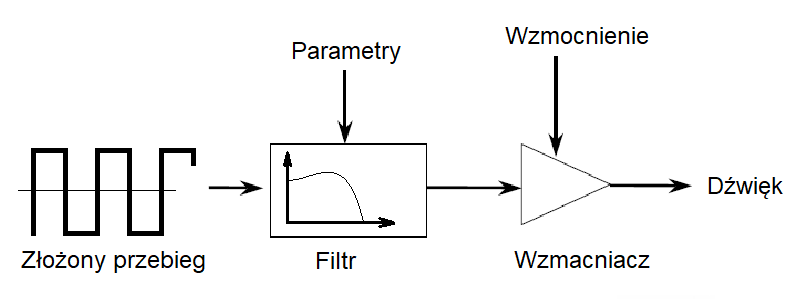
\includegraphics[width=12cm]{grafiki/sub_diagram}
	\captionsetup{justification=centering}
	\caption{Schemat blokowy dla metody subtraktywnej.}
	\label{rys:sub_diagram}
\end{figure}

Przykładowy wynik takiego działania przedstawiony jest na rysunku \ref{rys:sub_wykres1}.
\begin{figure}[H]
	\centering
	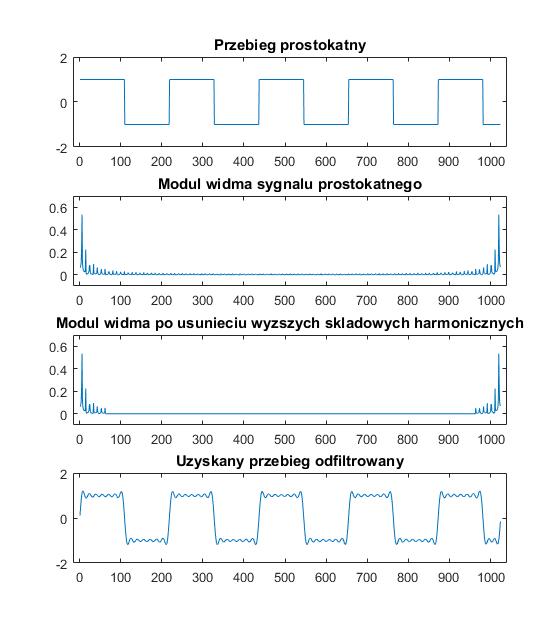
\includegraphics[width=12cm]{grafiki/sub_wykres1}
	\captionsetup{justification=centering}
	\caption{Zasada działania metody subtraktywnej.}
	\label{rys:sub_wykres1}
\end{figure}
Jak widać na rysunku \ref{rys:sub_wykres1}, na początku generowane jest 1024 próbek przebiegu prostokątnego. Następnie obliczane jest widmo tego sygnału. Z widma usuwane są wyższe składowe harmoniczne. Osiągnąć to można za pomocą filtracji idealnym filtrem dolnoprzepustowym. Przykład takiego filtra opisanego w dziedzinie częstotliwości jako
\begin{equation} \label{equ:sub_lowpass}
H(\omega)=\left \{\begin{array}{ r l }
1, & \quad \text{$dla$ } \omega \leqslant \omega_{gr}\\
0, & \quad  \text{$dla$ } \omega > \omega_{gr}
\end{array}
\right.
\end{equation}
\begin{tabular}{ l l l l}
	gdzie: & $\omega$ &  - & pulsacja, \\
	&	$\omega_{gr}$ & - &  pulsacja graniczna filtra,\\
\end{tabular} \\ \\
przedstawiono na rysunku \ref{rys:sub_lowpass}. Pulsacja graniczna filtra to taka pulsacja, powyżej której wzmocnienie jest mniejsze niż 3 dB w stosunku do pasma przepustowego. W przypadku idealnym wzmocnienie zmienia się skokowo z 1 na 0 dokładnie na pulsacji granicznej. W przedstawionym przykładzie pulsacja graniczna wynosi około 6283 rad/s, co zgodnie ze wzorem
\begin{equation} \label{equ:sub_frequency}
f = \frac{\omega}{2 \pi}
\end{equation}
daje częstotliwość równą 1000 Hz.
\begin{figure}[H]
	\centering
	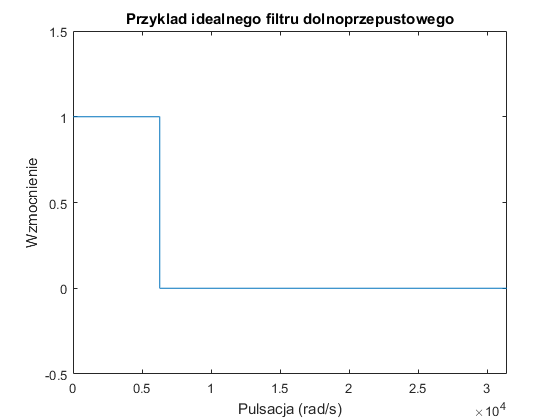
\includegraphics[width=8cm]{grafiki/sub_lowpass}
	\captionsetup{justification=centering}
	\caption{Idealny filtr dolnoprzepustowy.}
	\label{rys:sub_lowpass}
\end{figure}

Aby zadany sygnał poddać przetworzeniu za pomocą filtra, należy wykonać operację splotu:
\begin{equation} \label{equ:sub_splot}
y(t)= h(t)*x(t) = \int_{0}^{t} h(\tau)x(t-\tau)d\tau
\end{equation}
\begin{tabular}{ l l l l}
	gdzie: & $y(t)$ &  - & wynik splotu, \\
	&	$h(t)$ & - &  odpowiedź impulsowa filtra,\\
	&	$x(t)$ & - &  filtrowany sygnał,\\
	
\end{tabular} \\ \\
który w przypadku dyskretnym jest zdefiniowany jako:
\begin{equation} \label{equ:sub_splot_dyskretny}
y[n]= h[n]*x[n] = \sum_{k=-\infty}^{\infty} h[k]x[n-k]
\end{equation}
% OPISAĆ!!!!

Jedną z własności przekształcenia Fouriera jest to, że operacji splotu w dziedzinie czasu odpowiada operacja mnożenia w dziedzinie częstotliwości
\begin{equation} \label{equ:sub_splot_twierdzenie}
\mathcal{F}\{y(t)\} = \mathcal{F}\{h(t)*x(t)\} = H(\omega) X(\omega)
\end{equation}
\begin{tabular}{ l l l l}
	gdzie: & $\mathcal{F}\{y(t)\}$ &  - & transformata Fouriera wyniku splotu, \\
	&	$ H(\omega)$ & - &  transformata Fouriera odpowiedzi impulsowej filtra,\\
	&	$X(\omega)$ & - &  transformata Fouriera filtrowanego sygnału.\\
	
\end{tabular} \\ \\
Analogicznie, dla przypadku dyskretnego:
\begin{equation} \label{equ:sub_splot_twierdzenie_dyskretne}
\mathcal{F}\{y[n]\} = \mathcal{F}\{h[n]*x[n]\} = H(k) X(k).
\end{equation}
\begin{tabular}{ l l l l}
	gdzie: & $ H(k)$ & - &  dyskretna transformata Fouriera odpowiedzi impulsowej filtra,\\
	&	$X(k)$ & - &  dyskretna transformata Fouriera filtrowanego sygnału.\\
	
\end{tabular} \\ \\
Oznacza to, że równoważnym do działania opisanego w (\ref{equ:sub_splot_dyskretny}) jest:
\begin{equation} \label{equ:sub_splot_dyskretny2}
y[n] = \mathcal{F}^{-1}\{ H(k) X(k)\} 
\end{equation}
Zatem z przefiltrowanego widma, za pomocą odwrotnej transformacji Fouriera, obliczany jest przebieg czasowy. W pokazanym przykładzie na rysunku \ref{rys:sub_wykres1}, w wyniku otrzymuje się sygnał prostokątny po filtracji dolnoprzepustowej.
\section{Implementacja syntezy subtraktywnej}
W przypadku syntezatorów analogowych, poszczególne bloki są realizowane za pomocą elementów elektronicznych takich jak oscylatory (VCO) oraz przestrajalne filtry. W syntezatorach cyfrowych implementacje mogą być różne, jednak muszą być na tyle wydajne obliczeniowo, aby dana platforma sprzętowa poradziła sobie z syntezą dźwięku w czasie rzeczywistym bez artefaktów dźwiękowych. W tym podrozdziale opisana zostanie obrana droga implementacji metody subtraktywnej na procesorze sygnałowym. 
Próbki sygnału są syntezowane w sposób blokowy. Blok danych składa się z $N=1024$ próbek.



\subsection{Generowanie przebiegu}
W dwóch tablicach o $N$ elementach przechowywane są kolejne próbki sygnału podstawowego, czyli sygnału bogatego w wyższe składowe harmoniczne. 
%Po dokonaniu filtracji i przesłaniu danych jednej z tablic do przetwornika cyfrowo-analogowego, do przetwornika trafiają próbki z drugiej tablicy. 
Dane są przesyłane do przetwornika DAC na przemian z jednej lub drugiej tablicy.
%POPRAWIĆ
W tym czasie w chwilowo nieużywanej tablicy należy wygenerować kolejne 1024 próbek sygnału. Trzeba przy tym pamiętać o odpowiednim przesunięciu fazowym, tak aby zachować ciągłość pomiędzy kolejnymi blokami przesyłanymi do przetwornika. Równanie (\ref{equ:sub_1}) opisuje sposób generowania przebiegu prostokątnego.

	\iffalse
	\begin{equation} \label{equ:sub_1}
	waveform[i]=\left \{\begin{array}{ r l }
	1, & \quad \text{$dla$ } \text{sin}(2\pi f\frac{k+i}{F_s}) > 0\\
	-1, & \quad  \text{$dla$ } \text{sin}(2\pi f\frac{k+i}{F_s}) \leqslant 0
	\end{array}
	\right.
	\end{equation}
	\fi
\begin{equation} \label{equ:sub_1}
\text{waveform[i]}=\text{sgn}(\text{sin}(2\pi f\frac{k+i}{F_s}))
%zmienic formatowanie waveform[i] na jakies sanserif(????) i bold
\end{equation}
\begin{tabular}{ l l l l}
	gdzie: & waveform &  - & tablica zmiennych typu float, \\
	&	$f$ & - &  pożądana częstotliwość generowanego przebiegu, \\
	&	$F_s$ & - & częstotliwość próbkowania,\\
	&	$i$ & - &  licznik iteracji, $i$ = 1, 2, 3, ..., N,\\
	&	$k$ & - &  licznik bloków.\\
\end{tabular} \\ \\
Po wyznaczeniu każdego bloku próbek, zwiększany jest licznik bloków $k$:
\begin{equation} \label{equ:sub_2}
k \gets k + N.
\end{equation}
Na rysunku \ref{rys:sub_waveform_blocks} pokazano dwie kolejne ramki próbek wygenerowanego przebiegu prostokątnego. Dzięki odpowiedniemu przesunięciu fazowemu fragmenty te, po przesyłaniu na przetwornik cyfrowo-analogowy, utworzą ciągły dźwięk - bez zakłóceń.
\begin{figure}[H]
	\centering
	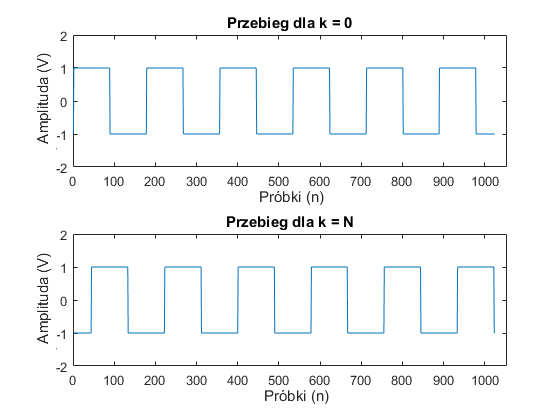
\includegraphics[width=12cm]{grafiki/sub_waveform_blocks}
	\captionsetup{justification=centering}
	\caption{Dwa kolejne bloki próbek przebiegu prostokątnego.}
	\label{rys:sub_waveform_blocks}
\end{figure}

\subsection{Efekt Gibbsa}\label{sec:gibbs}
Generowanie sygnału podstawowego opisane powyżej jest mało kosztowne obliczeniowo. W wyniku otrzymuje się wizualnie doskonały przebieg prostokątny. Jednak jego aproksymacja za pomocą skończonej liczby składowych sinusoidalnych jest niemożliwa. Oznacza to, że jego widmo nie będzie składało się tylko i wyłącznie ze składowych o częstotliwości przebiegu podstawowego i jej nieparzystych wielokrotności. Wynika to z braku spełnienia twierdzenia o próbkowaniu. 
%Powiedzieć, że tu nie jest spełnione twierdzenie o próbkowaniu
W widmie takiego sygnału pojawią się dodatkowe składowe w całym zakresie częstotliwości. Zjawisko to zostało przedstawione na rysunku \ref{rys:sub_gibbs1}.
\begin{figure}[H]
	\centering
	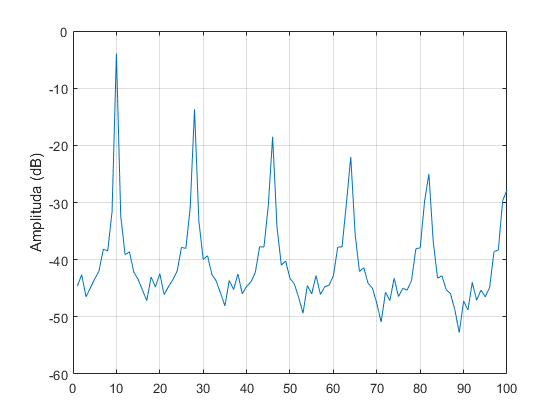
\includegraphics[width=8cm]{grafiki/sub_gibbs1}
	\captionsetup{justification=centering}
	\caption{Fragment widma amplitudowego idealizowanego sygnału prostokątnego.}
	\label{rys:sub_gibbs1}
\end{figure}

W celu wygenerowania sygnału prostokątnego, w którego widmie nie pojawiają się niechciane składowe, można wykorzystać wzór na aproksymację szeregiem Fouriera tego przebiegu:
\begin{equation} \label{equ:sub_gibbs}
\text{waveform[i]} = \sum_{p=1}^{P}\frac{1}{2p-1}\text{sin}(2\pi f(2p-1)  \frac{i}{F_s}).
\end{equation}
Wartość $P$ zależy od częstotliwości generowanego sygnału i opisuje ją zależność 
\begin{equation} \label{equ:sub_gibbs2}
P = \frac{F_s}{2f}.
\end{equation}
Dzięki takiemu wyborowi wartości $P$, w widmie pojawią się tylko składowe spełniające twierdzenie o próbkowaniu. Sygnał powstały w ten sposób przedstawiono na rysunku \ref{rys:sub_gibbs2}.
 \begin{figure}[H]
 	\centering
 	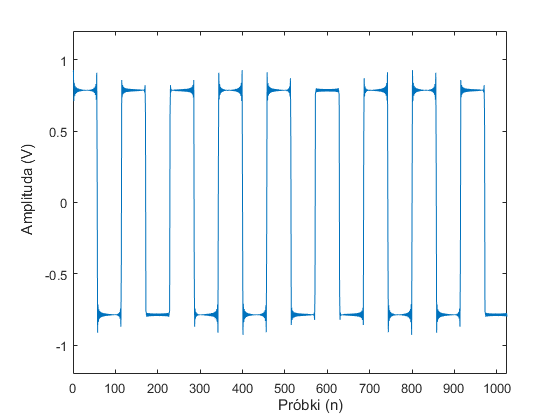
\includegraphics[width=8cm]{grafiki/sub_gibbs2}
 	\captionsetup{justification=centering}
 	\caption{Sygnał prostokątny aproksymowany szeregiem Fouriera.}
 	\label{rys:sub_gibbs2}
 \end{figure}

W pobliżu punktów nieciągłości widoczne są charakterystyczne oscylacje. Zjawisko to nazywane jest efektem Gibbsa. Pomimo gorszej prezencji w dziedzinie czasu, w widmie takiego sygnału nie pojawiają się niechciane składowe, co pokazano na rysunku \ref{rys:sub_gibbs3}.
\begin{figure}[H]
	\centering
	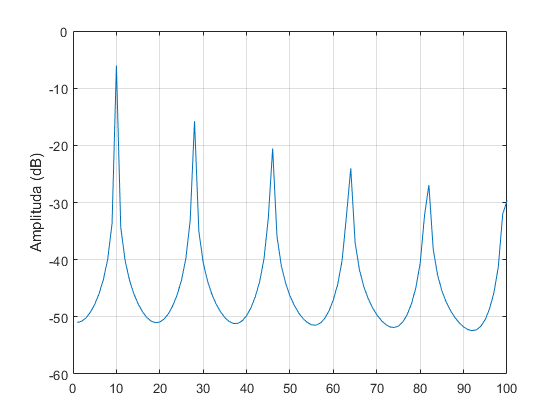
\includegraphics[width=8cm]{grafiki/sub_gibbs3}
	\captionsetup{justification=centering}
	\caption{Fragment widma amplitudowego aproksymowanego szeregiem Fouriera sygnału prostokątnego.}
	\label{rys:sub_gibbs3}
\end{figure}

Metoda generowania sygnałów przez aproksymację szeregiem Fouriera pozwala wyeliminować lekko słyszalne niechciane składowe. Jednak nie została ona wykorzystana ze względów na zbyt dużą złożoność obliczeniową. 

\subsection{DFT i filtracja sygnału}
Na podstawie wygenerowanych próbek przebiegu oblicza się DFT za pomocą algorytmu FFT. W wyniku otrzymuje się $N$ liczb zespolonych. Przechowywane są one w tablicy o rozmiarze $2N$ w taki sposób, że każdy element o indeksie parzystym to część rzeczywista próbki, a sąsiadujący z nią element o indeksie nieparzystym to część urojona tej próbki. Filtracja dokonywana jest poprzez wyzerowanie elementów o odpowiednich indeksach. Na przykład filtracja dolnoprzepustowa z częstotliwością graniczną o wartości 1400 Hz dokonywana jest według poniższego wzoru:
\begin{equation} \label{equ:sub_3}
\text{waveform}_{\text{fft}}\text{[i]}=\left \{\begin{array}{ r l }
0, & \quad  \text{dla } N - f_g \leqslant \frac{i}{2} \leqslant N + f_g \\
\text{waveform}_{\text{fft}}\text{[i]}, & \quad \text{w pozostałych przypadkach } 

\end{array}
\right.
\end{equation}
\begin{tabular}{ l l l l}
	gdzie: & $\text{waveform}_{\text{fft}}$ &  - & próbki transformaty Fouriera sygnału, \\
	&	$f_g$ & - &  częstotliwość przeliczona na indeksy w tablicy, $f_g = N - 2 \frac{1400N}{F_s} - 1$, \\
	&	$F_s$ & - & częstotliwość próbkowania,\\
	&	$i$ & - &  indeks, $i = 1, 2, 3, ..., 2N$.\\
\end{tabular} \\ \\

Efekt tego typu filtracji można zobaczyć na trzecim wykresie na \ref{rys:sub_wykres1}. W analogiczny sposób dokonuje się pozostałych filtracji: górnoprzepustowej, pasmo-przepustowej i pasmo-zaporowej.

\subsection{Zakładkowanie bloków danych}
Samo przesuwanie w fazie generowanych sygnałów opisane przez (\ref{equ:sub_2}) nie rozwiązuje wszystkich problemów. Jak widać na ostatnim wykresie na \ref{rys:sub_wykres1}, uzyskany sygnał na końcu ma niespodziewany przebieg. Po połączeniu następujących po sobie bloków próbek, otrzyma się nieciągłość pokazaną na rysunku \ref{rys:sub_zakladkowania_brak}.

\begin{figure}[H]
	\centering
	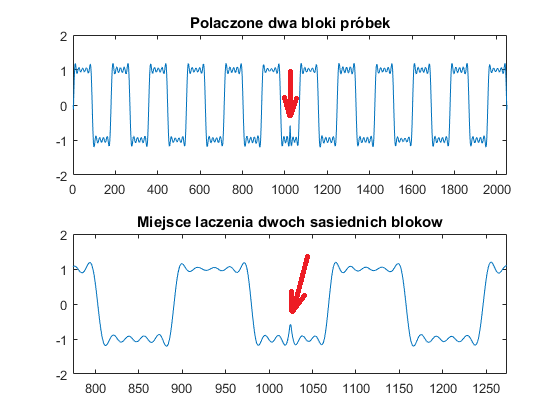
\includegraphics[width=12cm]{grafiki/sub_zakladkowania_brak}
	\captionsetup{justification=centering}
	\caption{Dwa kolejne bloki próbek przebiegu prostokątnego.}
	\label{rys:sub_zakladkowania_brak}
\end{figure}
Rozwiązaniem tego problemu jest zakładkowanie każdych dwóch sąsiednich porcji danych. Proces ten polega na nasunięciu pewnej liczby $m$ początkowych próbek następnego bloku, na $m$ końcowych próbek bloku bieżącego. W miejscach, gdzie ramki są na siebie nałożone, wartość sygnału obliczana jest jako średnia ważona z dwóch nachodzących na siebie elementów. Przy czym suma wag w każdej chwili czasu jest równa 1. Wagi $m$ ostatnich próbek bloku bieżącego maleją do zera, natomiast wagi $m$ pierwszych próbek bloku następnego narastają do jedynki. Najprostszym rozwiązaniem (a zatem efektywnym obliczeniowo) są wagi liniowe. Oznacza to, że wagi dla $m$ ostatnich lub pierwszych próbek bloku odpowiednio: liniowo maleją od 1 do 0 lub liniowo rosną od 0 do 1.
Nakładane na siebie próbki muszą odpowiadać sygnałowi w tej samej fazie, zatem należy zmodyfikować przesunięcie fazowe opisane przez (\ref{equ:sub_2}) do postaci:
\begin{equation} \label{equ:sub_4}
k \gets k + N - m.
\end{equation}
Porównanie zakładkowania dla różnych wartości $m$ przedstawiono na rysunku  \ref{rys:sub_overlaps}.
\begin{figure}[H]
	\centering
	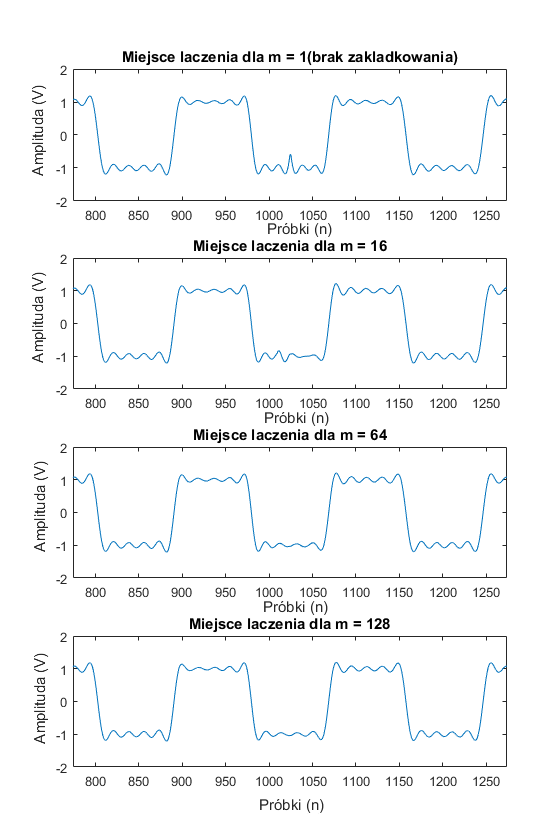
\includegraphics[width=10cm]{grafiki/sub_overlaps}
	\captionsetup{justification=centering}
	\caption{Wyniki zakladkowania przy zmiennej dlugosci zakladek.}
	\label{rys:sub_overlaps}
\end{figure}

Takie podejście wymusza użycie dwóch tablic ze zmiennymi typu float zawierającymi próbki sygnału, które będą przesyłane na przetwornik cyfrowo-analogowy. Wynika to z faktu, że w pewnych chwilach czasu, na DAC należy wysłać ważoną średnią próbek z dwóch różnych bloków. 

\subsection{Polifonia w syntezie subtraktywnej}
Powyższe rozważania dotyczyły syntezy pojedynczych tonów. Polifonię można osiągnąć wykonując opisane wcześniej operacje dla każdego naciśniętego klawisza instrumentu. Jednak aby zmniejszyć liczbę potrzebnych operacji wykonywanych na DSP, można wykorzystać własność liniowości przekształcenia Fouriera \cite{schafer}. Oznacza ona, że jeśli
 \begin{equation} \label{equ:sub_5}
 \mathcal{F}\{x_n\} = X_k
 \end{equation}
 oraz 
  \begin{equation} \label{equ:sub_6}
 \mathcal{F}\{y_n\} = Y_k
 \end{equation}
 wówczas
  \begin{equation} \label{equ:sub_7}
\mathcal{F}\{ax_n + by_n\} = aX_k + bY_k.
\end{equation} 
Dzięki temu nie trzeba przeprowadzać operacji całego toru syntezy dla każdego naciśniętego klawisza instrumentu. Można utworzyć sygnał będący sumą przebiegów podstawowych o odpowiednich częstotliwościach. Dopiero taki sygnał poddawany będzie dalszemu przetwarzaniu. Na rysunku \ref{rys:sub_linearity}	zobrazowana została własność liniowości przekształcenia Fouriera. Na pierwszych trzech wykresach pokazane zostały 3 przebiegi prostokątne o różnych częstotliwościach. W drugim rzędzie widnieją te przebiegi po przekształceniu przez taki sam filtr dolnoprzepustowy. W trzecim rzędzie znajduje się sygnał, który jest sumą początkowych przebiegów prostokątnych (przed filtracją). W ostatnim rzędzie pokazano sumę przefiltrowanych sygnałów oraz przefiltrowaną tym samym filtrem sumę sygnałów nieprzefiltrowanych. Przykład ten pokazuje, że obie drogi prowadzą do tych samych wyników.
\begin{figure}[H]
	\centering
	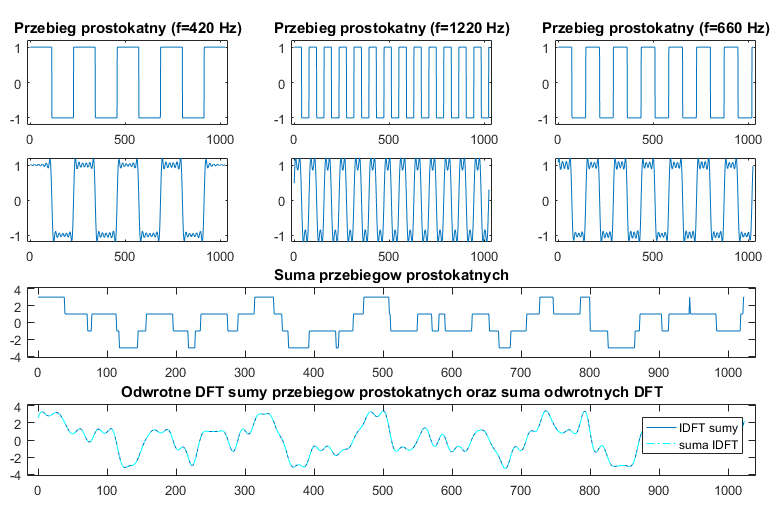
\includegraphics[width=16cm]{grafiki/sub_linearity}
	\captionsetup{justification=centering}
	\caption{Własność liniowości przekształcenia Fouriera.}
	\label{rys:sub_linearity}
\end{figure}

\section{Interfejs użytkownika}
Przy syntezie subtraktywnej, użytkownik powinien mieć możliwość samodzielnego wyboru przebiegów podstawowych generowanych przy naciskaniu klawiszy syntezatora oraz strojenia filtrów, które będą usuwać składowe harmoniczne. W przypadku filtrów idealnych, jedyne co użytkownik musi określić, to ich częstotliwości graniczne.
\begin{figure}[H]
	\centering
	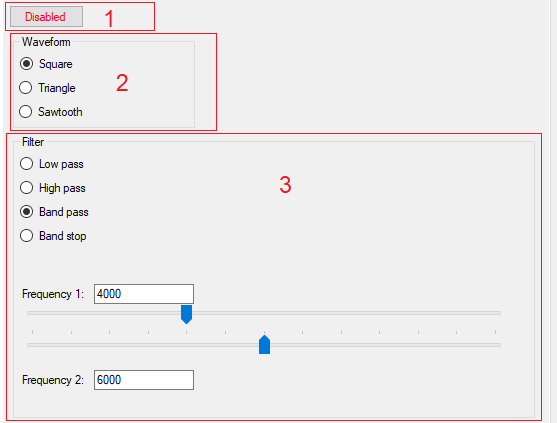
\includegraphics[width=12cm]{grafiki/sub_interface}
	\captionsetup{justification=centering}
	\caption{Interfejs użytkownika dla syntezy subtraktywnej.}
	\label{rys:sub_interface}
\end{figure}
Na rysunku \ref{rys:sub_interface} zaznaczono trzy sekcje wykonanego interfejsu dla syntezy subtraktywnej. W pierwszej z nich znajduje się przycisk, który służy do aktywacji tej metody syntezy dźwięku. Po naciśnięciu tego klawisza, DSP otrzymuje komunikat, po którym przechodzi w tryb syntezy subtraktywnej.

W sekcji drugiej znajdują się rodzaje przebiegów podstawowych wykorzystywane w syntezie. W tym samym czasie może być aktywny tylko jeden z nich. Zaznaczenie dowolnego z przebiegów zmienia w programie DSP odpowiednią flagę. Naciskanie klawiszy syntezatora będzie skutkowało generowaniem sygnałów podstawowych o kształcie wybranym za pomocą interfejsu użytkownika.

W trzeciej sekcji dokonuje się wyboru rodzaju filtra oraz suwaki pozwalające na wybór częstotliwości granicznych: dolnej, górnej lub obu jednocześnie - zależnie od wybranego rodzaju filtra. Podobnie jak przy wyborze rodzaju przebiegu podstawowego - tutaj również użytkownik zaznacza jedną z opcji. W zależności od wybranego filtra, odblokowane zostaną odpowiednie suwaki pozwalające zmieniać częstotliwości graniczne. Na przykład, dla filtra dolnoprzepustowego odblokowany zostanie tylko suwak dolny, gdyż to on odpowiada za częstotliwość graniczną górną. Natomiast dla filtra pasmo-przepustowego odblokowane zostaną oba suwaki, a pasmo przepustowe zawierać się będzie pomiędzy wskazaniem suwaka górnego - częstotliwości granicznej dolnej oraz suwaka dolnego - częstotliwości granicznej górnej.
Zmian częstotliwości można dokonywać na dwa sposoby:
\begin{itemize}
	\item za pomocą suwaków. W tym wypadku wartość ustawiona za pomocą suwaka zostanie automatycznie wpisana do pola tekstowego skojarzonego z tym suwakiem.
	\item Poprzez precyzyjne wpisanie wartości do pola tekstowego obok suwaka. W tej sytuacji suwak automatycznie się przesunie na pozycję odpowiadającą wpisanej wartości.
\end{itemize}

\section{Wyniki}
Zaimplementowana na DSP synteza subtraktywna dała dobre wyniki odsłuchowe. Zastosowany algorytm jest w stanie wygenerować do 12 różnych tonów jednocześnie. Jedynym defektem jest są lekko słyszalne dodatkowe harmoniczne opisane w części \ref{sec:gibbs}. Uzyskanie czystszego brzmienia wiąże się ze zwiększeniem złożności obliczeniowej, a co za tym idzie - zmniejszeniem liczby tonów, które mogą być generowane jednocześnie.
